\documentclass[nocover]{pset}
\usepackage{tikz-cd}
\pagestyle{fancy}
\fancyhf{}
\lhead{Forest Kobayashi}
\chead{Basic Category Theory}
\rhead{Math 196 -- Fall, 2018}
\rfoot{\thepage\ of \pageref{LastPage}}
\setlength{\headheight}{15.2pt}
\setlength{\headsep}{10pt}
\lfoot{Thursday, October 4th 2018}

\usepackage{graphicx}
\newcommand\sbullet[1][.5]{\mathbin{\vcenter{\hbox{\scalebox{#1}{$\bullet$}}}}}


\begin{document}

\begin{center}
  {\scshape \Large Misc.\ Categories and Introduction to Universals}

  {\scshape Lecture 3}
\end{center}
\vspace{-.1cm}
\hrulefill
\begin{adjustwidth}{1em}{1em}
  \section{Introduction}
  Recall the definition of a natural transformation.
  \begin{definition}[Natural Transformation]
    Let $\mb{B,C}$ be categories, and let $\mc{F, G} : \mb{C} \to
    \mb{D}$. Let $\eta$ be called a \emph{natural transformation} if
    \begin{enumerate}[label=\roman*)]
      \item For all $c \in \mb C$, $\eta$ assigns a morphism $\eta_c :
        \mc{F}_o(c) \to \mc{G}_o(c)$ (known as the \emph{component} of
        $\eta$ at $c$), such that
      \item $\forall f: c \to c' $, $\eta_{c'} \circ \mc{F}_a(f) =
        \mc{G}_a(f) \circ \eta_{c'}$
    \end{enumerate}
  \end{definition}
  when we first introduced natural transformations, we hinted that
  natural transformations can be thought of as morphisms on a category
  with functors as the objects. We return to this topic now, seeking a
  more formal understanding.
  \begin{definition}[Bullet composition]
    Let $\mb{C,B}$ be categories, and let $\mc{R,S,T}, \ldots : \mb C
    \to \mb B$. Then let $\sigma : \mc{R} \xrightarrow{\sbullet} \mc{S}$
    and $\tau : \mc{S} \xrightarrow{\sbullet} \mc{T}$ be natural
    transformations. Then define $\tau \sbullet \sigma : \mc{R}
    \xrightarrow{\sbullet} \mc{T}$ such that $\forall c \in \mb C$, we
    have
    \[
      \pn{\tau \sbullet \sigma}_c = \tau_c \circ \sigma_c.
    \]
    Then the composite $\tau \sbullet \sigma$ is natural.
  \end{definition}
  $\sbullet$ is associative, and for each $\mc T$, has an identity
  transformation, namely $1_{\mc T} : \mc T \to \mc T$, with $c
  \mapsto 1_{\mc T c}$. Thus, the functors themselves carry the
  structure of a category.
  \begin{definition}[Functor Category]
    Let $\mb{B,C}$ be categories. Then we construct a \emph{functor
      category} $\mb B^{\mb C} = \mrm{Funct}(\mb C, \mb B)$ with
    objects
    \[
      \ob\pn{\mb B^{\mb C}} = \set{T : \mb C \to \mb B}
    \]
    and morphisms
    \[
      \homm\pn{\mb B^{\mb C}} = \set[big]{ \tau \MID \tau : \mc{S}
        \xrightarrow{\sbullet} \mc T,\ \tau \text{ is natural}}.
    \]
  \end{definition}
  with composition defined by $\sbullet$. We'll consider a few
  examples:
  \begin{enumerate}
    \item Let $X$ a finite set, and $\mb B$ a category. Then $\mb
      B^{X}$ is the set of all functions from $X$ to $\mb B$.
  \end{enumerate}



  One might wonder whether we can find another definition of
  composition that


  \section{Comma Categories}
  Comma categories will play a large role in studying Adjoint functors
  in the future, so we'll take some time here to discuss them in
  detail. Essentially, Comma categories serve as a way of connecting
  two functors that share the same codomain category, by constructing
  the category of morphisms between their images.
  \begin{definition}[Comma Category]
    Let $\mb C,D,E$ be categories, and let $\mc F,G$ be functors with
    $\mc F : D \to C$, and $\mc G : E \to C$. Then the \emph{comma
      category}, denoted by
    \[
      \pn{\mc{F} \downarrow \mc{G}} \quad \text{or} \quad \pn{\mc{F, G}}
    \]
    is defined as follows:
    \[
      \ob\pn{\pn{\mc F \downarrow \mc G}} = \set{\ip{d,e,f} \MID d \in
        \ob(\mb D), e \in \ob(\mb E), f : \mc{F}_o(d) \to
        \mc{G}_o(e)},
    \]
    which can be expressed diagramatically by
    \begin{figure}[H]
      \centering
      \begin{tikzpicture}
        \node (fd) at (0,1) {$\mc{F}_o(d)$};
        \node (ge) at (0,-1) {$\mc{G}_o(e)$};
        \draw[->] (fd) -- (ge) node[midway, right] {$f$};
      \end{tikzpicture}
      \caption{Objects of $\pn{\mc F \downarrow \mc G}$}
    \end{figure}
    and
    \[
      \homm\pn{\pn{\mc F \downarrow \mc G}} = \set{\ip{g,h} \MID g : d
      \to d', h : e \to e'}
    \]
    such that
    \begin{figure}[H]
      \centering
      \begin{tikzpicture}
        \node (fd) at (0,1) {$\mc{F}_o(d)$};
        \node (ge) at (0,-1) {$\mc{G}_o(e)$};
        \node (fpd) at (2.5,1) {$\mc{F}_o(d')$};
        \node (gpe) at (2.5,-1) {$\mc{G}_o(e')$};
        \draw[->] (fd) -- (ge) node[midway, left] {$f$};
        \draw[->] (fpd) -- (gpe) node[midway, right] {$f'$};
        \draw[->] (ge) -- (gpe) node[midway, above] {$\mc{G}_a(h)$};
        \draw[->] (fd) -- (fpd) node[midway, above] {$\mc{F}_a(g)$};
      \end{tikzpicture}
      \caption{Morphisms of $\pn{\mc F \downarrow \mc G}$}
    \end{figure}
    commutes.
  \end{definition}
  Essentially, we're
\end{adjustwidth}


\end{document}
